\documentclass{paper}

%\usepackage{times}
\usepackage{epsfig}
\usepackage{graphicx}
\usepackage{amsmath}
\usepackage{amssymb}
\usepackage{color}
\usepackage{caption}
\usepackage{subcaption}

% load package with ``framed'' and ``numbered'' option.
%\usepackage[framed,numbered,autolinebreaks,useliterate]{mcode}

% something NOT relevant to the usage of the package.
\setlength{\parindent}{0pt}
\setlength{\parskip}{18pt}






\usepackage[latin1]{inputenc} 
\usepackage[T1]{fontenc} 

\usepackage{listings} 
\lstset{% 
   language=Matlab, 
   basicstyle=\small\ttfamily, 
} 



\title{Report for assignment 1}



\author{Moser Stefan\\09-277-013}
% //////////////////////////////////////////////////


\begin{document}



\maketitle

\section{Photometric Stereo (Due on 29/10/2013)}

In this assignment, we first retrieve the light directions of twelve images
of a chrome sphere. Then we use these light directions to compute the
normals, albedo and depth of 12 images of a scene that were taken under the
same lighting conditions. We assume, the chrome sphere does specular
 reflection, while the other scenes only do diffuse reflection (as
lambertian materials).

\subsection{Calculating the light direction} 
We know, that every point on the sphere must satisfy
\begin{equation}
	r^2 = x^2 + y^2 + z^2
\label{eq:sphere_coord}
\end{equation}
for the cartesian representation of a sphere as $(x,y,z)^T$ with the radius $r$. We can deploy this constraint, by bringing the bright
 highlight into the sphere coordinate system. This is simply done 
 by subtracting the center of the sphere. The variables used in eq. \ref{eq:light_direction} are:
\begin{itemize}
\item The 2D coordinates of the light source $i$'s highlight on the sphere, named $p_i$. It is computed as centroid of all points above a certain brightness threshold
\item The 2D coordinates of the centre of the sphere $c$, computed as the centroid of the mask.
\end{itemize}
\begin{equation}
	n_i = 
	\left[ 
	\begin{array}{c}
	(p_i - c)_x \\
	(p_i - c)_y \\
	-\sqrt{r^2 - (p_i - c)_x^2 - (p_i - c)_y^2}
\end{array} 
\right] 
\label{eq:light_direction}
\end{equation}
For the z coordinate, eq. \ref{eq:sphere_coord} can be solved for z. The negative solution is the correct choice, since it is the one pointing towards the camera.

Once the normal at the lights highlight are retrieved, they can be used with ray reflection to get the direction towards the light
\begin{equation}
	L_i = d - 2(d\cdot \hat{n}_i)\hat{n}_i
\end{equation}
with $\hat{n}_i$ being the normalized vector of $n_i$ and $d$ the direction of a light ray from the camera towards the sphere.
The assumption given in the assignment is, 
that every ray originating from the camera has direction $d = (0,0,1)$ for every point of the image.

All light directions $L_i$ can be assembled into a matrix $\mathbf{L}$. Here the
transposed version is shown, since it is easier to fit on a page.
\begin{align*}
\mathbf{L}^T= 
\left[ 
\begin{array}{cccccccccccccc}
0.4507 & -0.4230 & -0.7861 \\ 0.2180 & -0.1229 & -0.9682 \\ -0.0345 & -0.1577 & -0.9869 \\ -0.0854 & -0.3983 & -0.9133 \\ -0.2897 & -0.4593 & -0.8397 \\ -0.1012 & -0.5080 & -0.8554 \\ 0.2540 & -0.3823 & -0.8885 \\ 0.0908 & -0.3885 & -0.9170 \\ 0.1856 & -0.3014 & -0.9353 \\ 0.0794 & -0.2990 & -0.9510 \\ 0.1158 & -0.0415 & -0.9924 \\ -0.1295 & -0.3261 & -0.9364 
\end{array} 
\right] 
\end{align*}
They are fairly close to the defaults given. The mean squared error over all normalized directions is 0.0217.

\subsection{Computing Surface Normals and Grey Albedo}


For computing the grayscale albedo, I first reduced the color information to a single channel by computing the luminance $\ell$
\begin{equation}
	\ell = c_\text{r} \cdot 0.299 + 
		c_\text{g} \cdot 0.587 + 
		c_\text{b} \cdot 0.114
\end{equation}
for each image. 

In the lecture it was shown, that we can compute the normals by solving
\begin{align*}
	 I &= S\tilde{n} \\
	 S^TI &= S^T\tilde{n} \\
	 \tilde{n} &= (S^TS)^{-1}S^TI
\end{align*}
with 
\begin{itemize}
	\item $I$ a vector of the luminance values of the 
	inspected pixel for all $n$ images
	\item $S$ a matrix of all light directions, with each row
	having the light direction of the corresponding image.
	\item $\tilde{n}$ the normal direction (not unit size)
\end{itemize}
We know that we can obtain the grayscale albedo $\rho$ by taking the length of $\tilde{n}$
\begin{equation}
	n = \frac{\tilde{n}}{\rho}
\end{equation}
Once we know the normals, we can use them to compute the color albedo $a$, using
\begin{align*}
	I &= a(n \cdot L) \\
	(n \cdot L)^{-1} I &= a
\end{align*}
on every pixel.

\begin{figure}[h!]
        \centering
        \begin{subfigure}{0.3\textwidth}
                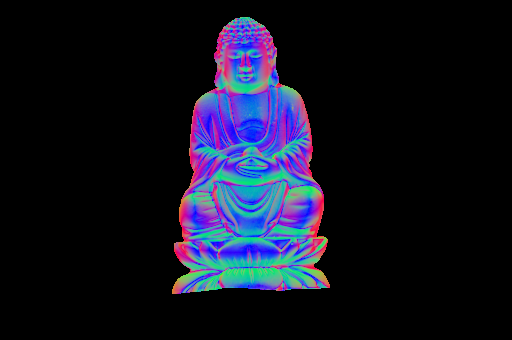
\includegraphics[width=\textwidth]{report_fig/buddha_n}
        \end{subfigure}
        ~ 
        \begin{subfigure}{0.3\textwidth}
                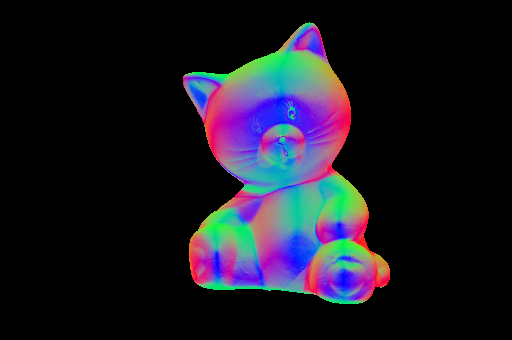
\includegraphics[width=\textwidth]{report_fig/cat_n}
        \end{subfigure}
        ~ 
        \begin{subfigure}{0.3\textwidth}
                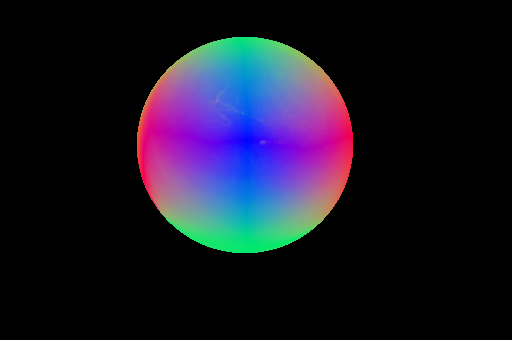
\includegraphics[width=\textwidth]{report_fig/gray_n}
        \end{subfigure}
        % second row
        \begin{subfigure}{0.3\textwidth}
                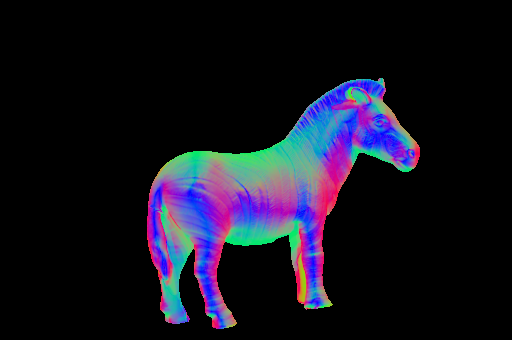
\includegraphics[width=\textwidth]{report_fig/horse_n}
        \end{subfigure}
        ~ 
        \begin{subfigure}{0.3\textwidth}
                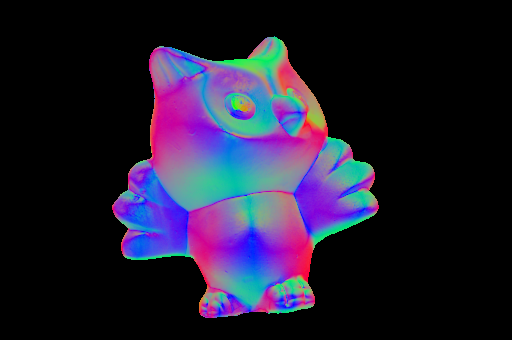
\includegraphics[width=\textwidth]{report_fig/owl_n}
        \end{subfigure}
        ~ 
        \begin{subfigure}{0.3\textwidth}
                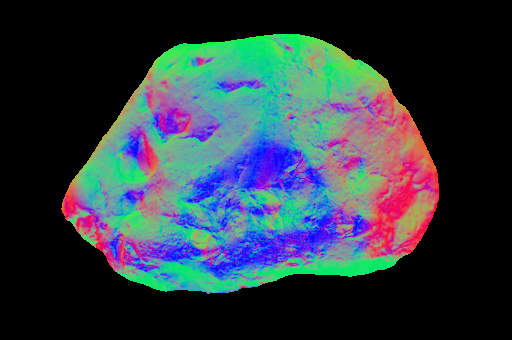
\includegraphics[width=\textwidth]{report_fig/rock_n}
        \end{subfigure}
        \caption{The normals visualized for every scene. For transforming
         them into rgb range, I took the absolute value. The x-axis
         is pointing to the right, the y-axis up and the z-axis towards
         the reader. The background 
         (where the mask is zero) is shown black. }
        \label{fig:normals}
\end{figure}
\begin{figure}[h!]
        \centering
        \begin{subfigure}{0.3\textwidth}
                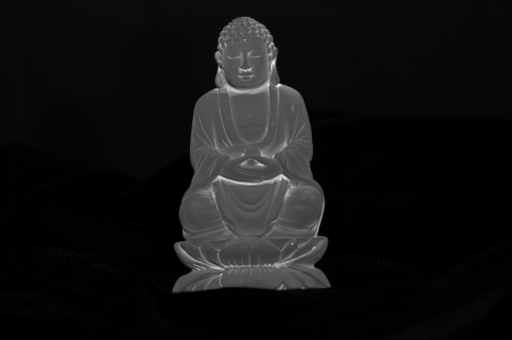
\includegraphics[width=\textwidth]{report_fig/buddha_a}
        \end{subfigure}
        ~ 
        \begin{subfigure}{0.3\textwidth}
                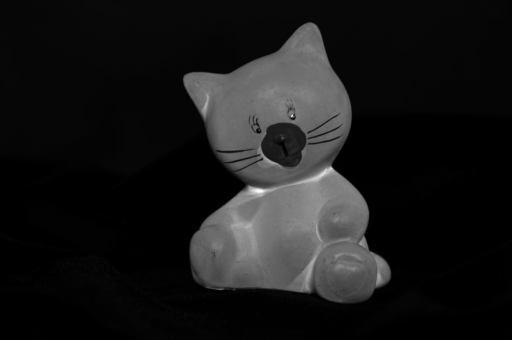
\includegraphics[width=\textwidth]{report_fig/cat_a}
        \end{subfigure}
        ~ 
        \begin{subfigure}{0.3\textwidth}
                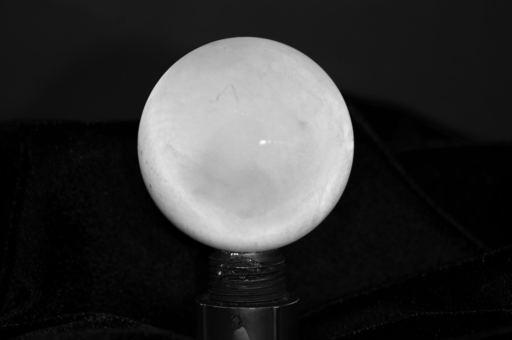
\includegraphics[width=\textwidth]{report_fig/gray_a}
        \end{subfigure}
        % second row
        \begin{subfigure}{0.3\textwidth}
                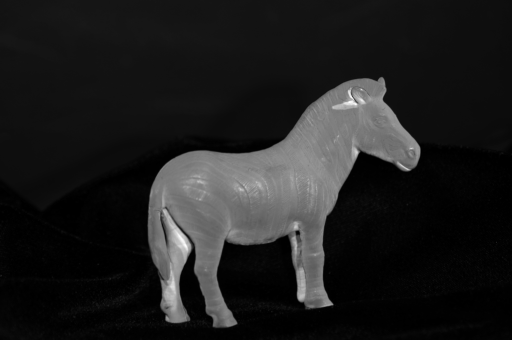
\includegraphics[width=\textwidth]{report_fig/horse_a}
        \end{subfigure}
        ~ 
        \begin{subfigure}{0.3\textwidth}
                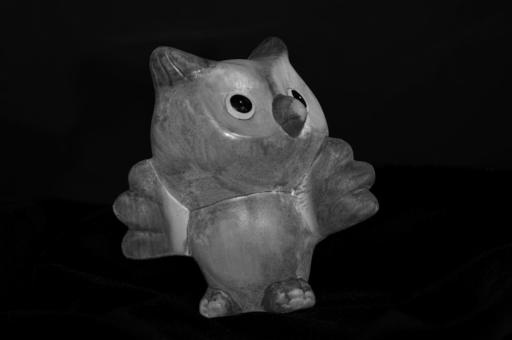
\includegraphics[width=\textwidth]{report_fig/owl_a}
        \end{subfigure}
        ~ 
        \begin{subfigure}{0.3\textwidth}
                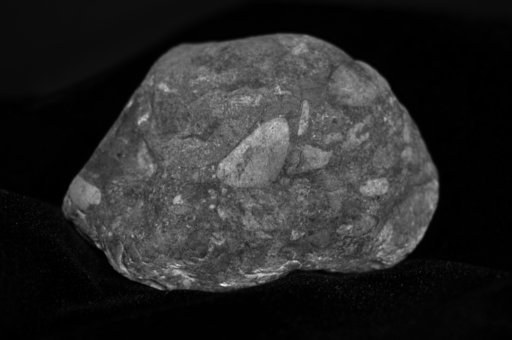
\includegraphics[width=\textwidth]{report_fig/rock_a}
        \end{subfigure}
        \caption{The grayscale albedo (luminance)}
        \label{fig:grayscale_albedo}
\end{figure}

\begin{figure}[h!]
        \centering
        \begin{subfigure}{0.3\textwidth}
                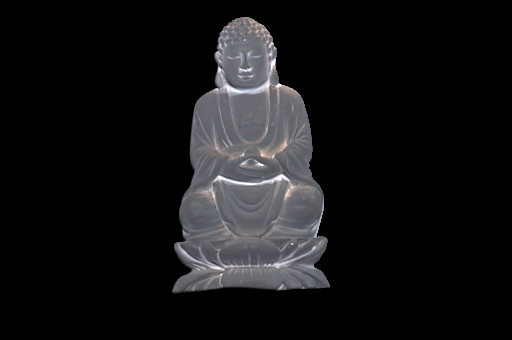
\includegraphics[width=\textwidth]{report_fig/buddha_ca}
        \end{subfigure}
        ~ 
        \begin{subfigure}{0.3\textwidth}
                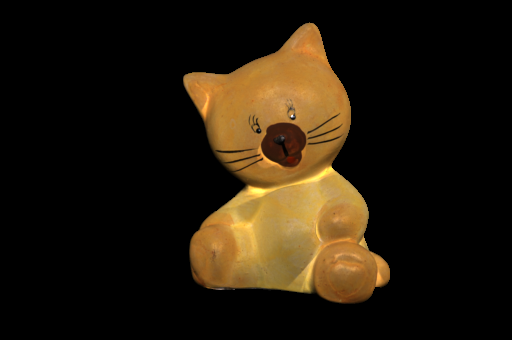
\includegraphics[width=\textwidth]{report_fig/cat_ca}
        \end{subfigure}
        ~ 
        \begin{subfigure}{0.3\textwidth}
                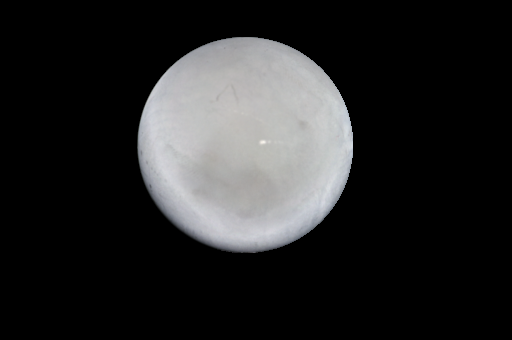
\includegraphics[width=\textwidth]{report_fig/gray_ca}
        \end{subfigure}
        % second row
        \begin{subfigure}{0.3\textwidth}
                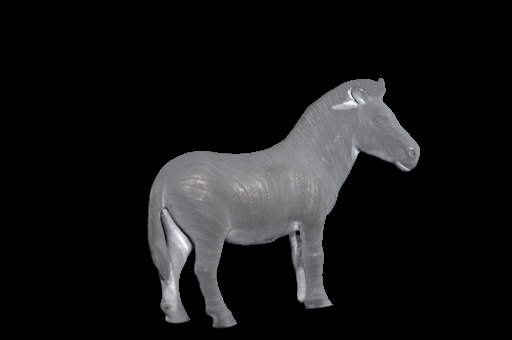
\includegraphics[width=\textwidth]{report_fig/horse_ca}
        \end{subfigure}
        ~ 
        \begin{subfigure}{0.3\textwidth}
                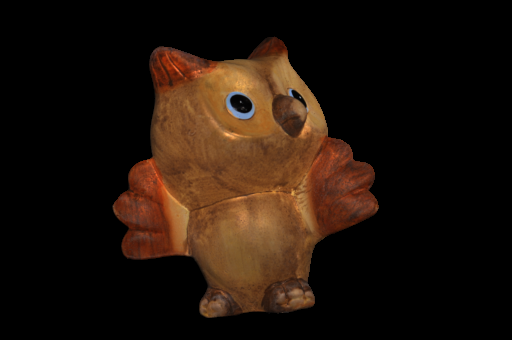
\includegraphics[width=\textwidth]{report_fig/owl_ca}
        \end{subfigure}
        ~ 
        \begin{subfigure}{0.3\textwidth}
                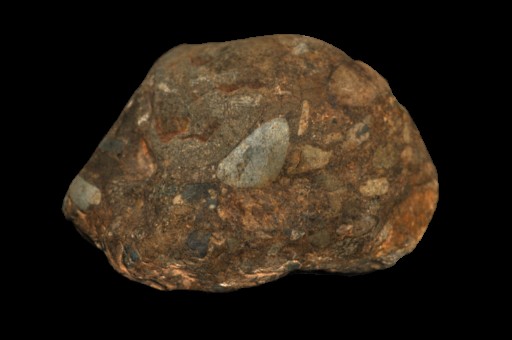
\includegraphics[width=\textwidth]{report_fig/rock_ca}
        \end{subfigure}
        \caption{The color albedo. The buddha, sphere and horse
        do in fact have a gray albedo, so there is not too much
        of a difference to the grayscale albedo.}
        \label{fig:color_albedo}
\end{figure}

\subsection{Surface Fitting}

We are looking for a way, to express the surface depth as function of the normal. The surface $S$ can be defined as with the depth as function of the other 
coordinates, as in $S(X,Y)=(X,Y,Z(X,Y))^T$. Next, we define the surface tangent
vectors in $X, Y$ direction at any point as partial derivatives
\begin{equation}
\begin{aligned}
	\textbf{t}_X &= \frac{\partial\textbf{S}}{\partial X} = (1, 0, Z_X)^T \\
	\textbf{t}_Y &= \frac{\partial\textbf{S}}{\partial Y} = (1, 0, Z_Y)^T
\end{aligned}
\label{eq:tangents}
\end{equation}
Since the normal can be expressed as normalized cross product of two tangential vectors, we know that
\begin{equation}
\begin{aligned}
	n(X,Y) &= \frac{\textbf{t}_X \times \textbf{t}_Y}
					{||\textbf{t}_X \times \textbf{t}_Y||} \\
		   &= \frac{(Z_X, Z_Y, -1)^T}{||(Z_X, Z_Y, -1)||}
\end{aligned}
\end{equation}
Further, the derivatives of the unknown depths can be approximated by
\begin{equation}
\begin{aligned}
	Z_X &\approx Z(x + 1, y) - Z(x,y) \\
	Z_Y &\approx Z(x, y + 1) - Z(x,y)	
\end{aligned}
\label{eq:approx}
\end{equation}
These approximations can be used to express the tangent vectors 
defined in eq. \ref{eq:tangents}. Since we know, that the normal and the tangent vector are perpendicular to each other, we can
formulate the constraint
\begin{equation}
\begin{aligned}
	\textbf{t}_X(x,y) \cdot n(x,y) = 0 \\
	\textbf{t}_Y(x,y) \cdot n(x,y) = 0
\end{aligned}
\end{equation}
This can be transformed to
\begin{equation}
\begin{aligned}
	(Z(x+1,y) - Z(x,y)) \cdot n(x,y)_z &= -n(x,y)_x \\
	(Z(x,y+1) - Z(x,y)) \cdot n(x,y)_z &= -n(x,y)_y 
\end{aligned}
\end{equation}
Now we have many linear equations, fill a whole matrix with this stuff, then solve.
This reduces the space of solutions to $Z(x,y) + c$ for any constant $c$. To reduce
it to one unique solution, an additional constraint in the form of 
\begin{equation}
	Z(x_0, y_0) = 0
\end{equation}
must be defined for a single pixel $(x_0, y_0)$. I choose to set the pixel in the top left to $Z(0,0) = 0$. An alternative I explored 
would be to set the depth of all pixels just outside the object boarder to $0$
\subsubsection{Results}
A successful reconstruction of the surface is never guaranteed, but having more images with 
more diverse light directions is one way to optimize the result. With more images,
the impact of self occlusion and noise is reduced. The depth map of the scenes
given for this assignment can be seen in figure \ref{fig:depth}.
\begin{figure}[h!]
        \centering
        \begin{subfigure}{0.3\textwidth}
                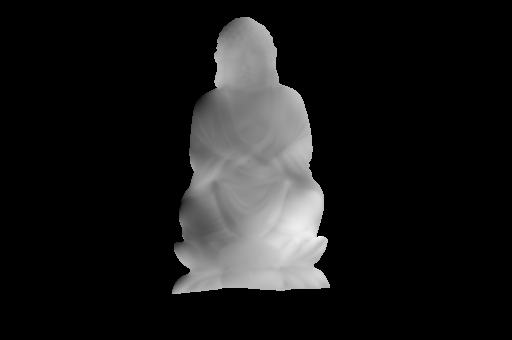
\includegraphics[width=\textwidth]{report_fig/buddha_d}
        \end{subfigure}
        ~ 
        \begin{subfigure}{0.3\textwidth}
                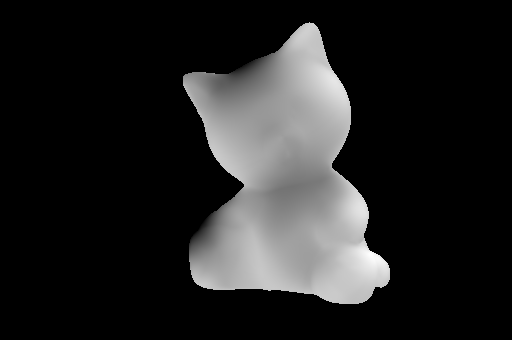
\includegraphics[width=\textwidth]{report_fig/cat_d}
        \end{subfigure}
        ~ 
        \begin{subfigure}{0.3\textwidth}
                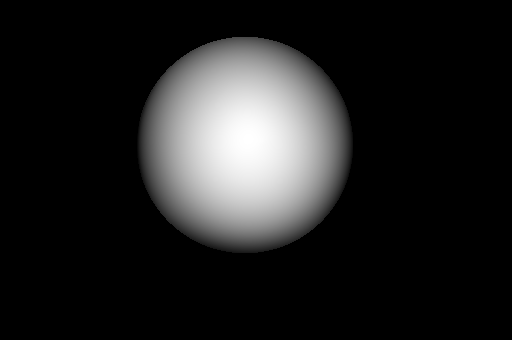
\includegraphics[width=\textwidth]{report_fig/gray_d}
        \end{subfigure}
        % second row
        \begin{subfigure}{0.3\textwidth}
                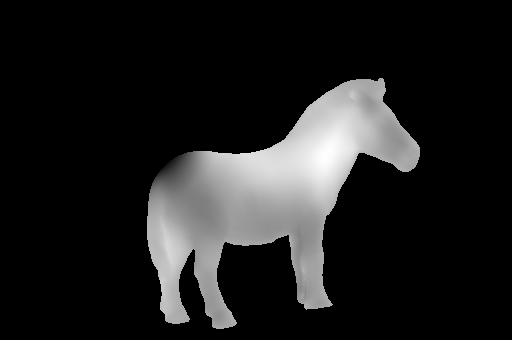
\includegraphics[width=\textwidth]{report_fig/horse_d}
        \end{subfigure}
        ~ 
        \begin{subfigure}{0.3\textwidth}
                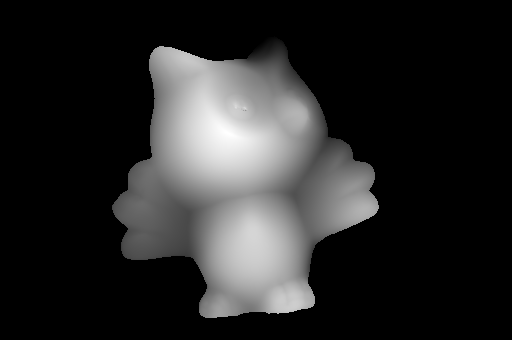
\includegraphics[width=\textwidth]{report_fig/owl_d}
        \end{subfigure}
        ~ 
        \begin{subfigure}{0.3\textwidth}
                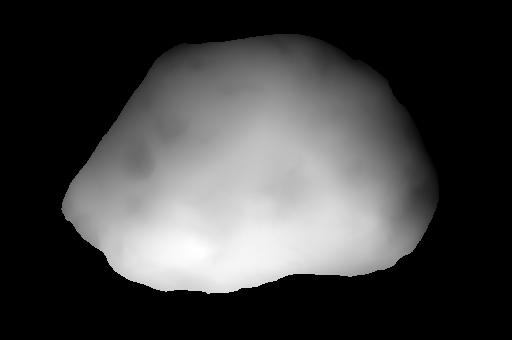
\includegraphics[width=\textwidth]{report_fig/rock_d}
        \end{subfigure}
        \caption{The depth. Brighter means closer to the camera.
        The background is set to black.}
        \label{fig:depth}
\end{figure}

\subsubsection{Failure cases}
\begin{itemize}
\item Materials are assumed to reflect light as a lambertian material would. 
If the material does have specular highlights, this method will fail. The eye of the owl
scene does have a visible artifacts due to this.

\item Self occlusion renders
this method difficult, since this methods does not handle shadows. This is visible around
the neck of the cat scene.

\item Inter reflection is not handled. The scenes presented in this report
do not contain such an example.

\item The surface must be sufficiently smooth, or the approximation from eq. \ref{eq:approx} will not be correct.
Objects with many sharp edges would not give a good result.
\end{itemize}
\end{document}